\section{Processus de reconfiguration} 

\begin{frame}{Processus de conception de reconfiguration existant}
\begin{figure}
\begin{subfigure}[b]{0.45\textwidth} % "0.45" donne ici la largeur
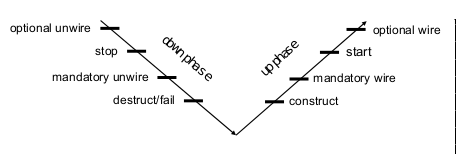
\includegraphics[width=5cm, height=3.8cm]{imgs/boyer_protocole}
\caption{Automatique, \emph{Boyer et al, 2017}}\label{fig:orchid}
\end{subfigure}
\begin{subfigure}[b]{0.45\textwidth} % "0.45" donne ici la largeur
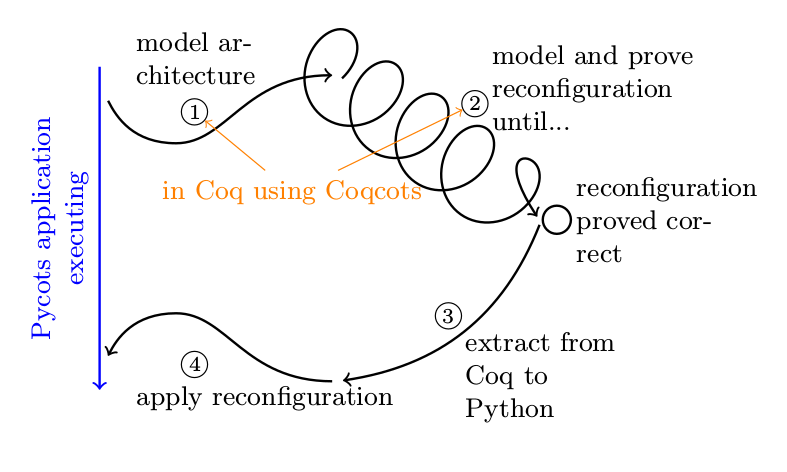
\includegraphics[width=5cm]{imgs/buisson_approche}\\
\caption{Manuelle \emph{Buisson et al, 2017}}\label{fig:orchid}
\end{subfigure}
\end{figure}
\end{frame}

\begin{frame}{Proposition d'un processus de reconfiguration}
\begin{columns}
\begin{column}{0.6\textwidth}
\begin{figure}
\centering
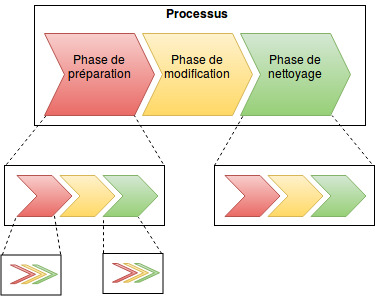
\includegraphics[width=0.9\textwidth]{imgs/phases-de-reconfiguration.jpg}
\end{figure}
\end{column}
\begin{column}{0.4\textwidth}
\begin{block}{}
\underline{\textbf{Phase de préparation}} : application de modification transitoire
\end{block}
\begin{block}{}
\underline{\textbf{Phase de modification}} : application actions souhaitées de reconfiguration
\end{block}
\begin{block}{}
\underline{\textbf{Phase de nettoyage}} : retourne le système vierge des modifications
liées à la reconfiguration
\end{block}
\end{column}
\end{columns}
\end{frame}

\begin{frame}{Utilisation des patrons de reconfiguration}
\begin{enumerate}
\item \underline{\textbf{Analyse}} Le processus s'appuie sur les patrons de reconfiguration. Dans un
premier temps, l'architecte analyse les modifications à apporter.
\item \underline{\textbf{Décision}}  il utilise le catalogue de patron pour identifier les problèmes qu'il
peut rencontrer et comment les résoudre. ou il définit un nouveau
patron.
\item \underline{\textbf{Récursion}} Dans le cas, ou le solution n'est pas directement applicable alors il
peut décider d'une nouvelle itération
\end{enumerate}
\end{frame}
